\documentclass[ignorenonframetext,]{beamer}
\setbeamertemplate{caption}[numbered]
\setbeamertemplate{caption label separator}{: }
\setbeamercolor{caption name}{fg=normal text.fg}
\beamertemplatenavigationsymbolsempty
\usepackage{lmodern}
\usepackage{amssymb,amsmath}
\usepackage{ifxetex,ifluatex}
\usepackage{fixltx2e} % provides \textsubscript
\ifnum 0\ifxetex 1\fi\ifluatex 1\fi=0 % if pdftex
  \usepackage[T1]{fontenc}
  \usepackage[utf8]{inputenc}
\else % if luatex or xelatex
  \ifxetex
    \usepackage{mathspec}
  \else
    \usepackage{fontspec}
  \fi
  \defaultfontfeatures{Ligatures=TeX,Scale=MatchLowercase}
\fi
% use upquote if available, for straight quotes in verbatim environments
\IfFileExists{upquote.sty}{\usepackage{upquote}}{}
% use microtype if available
\IfFileExists{microtype.sty}{%
\usepackage{microtype}
\UseMicrotypeSet[protrusion]{basicmath} % disable protrusion for tt fonts
}{}
\newif\ifbibliography
\hypersetup{
            pdftitle={Implementing Machine Learning},
            pdfauthor={John D. Lee and Linda Ng Boyle},
            pdfborder={0 0 0},
            breaklinks=true}
\urlstyle{same}  % don't use monospace font for urls
\usepackage{color}
\usepackage{fancyvrb}
\newcommand{\VerbBar}{|}
\newcommand{\VERB}{\Verb[commandchars=\\\{\}]}
\DefineVerbatimEnvironment{Highlighting}{Verbatim}{commandchars=\\\{\}}
% Add ',fontsize=\small' for more characters per line
\usepackage{framed}
\definecolor{shadecolor}{RGB}{248,248,248}
\newenvironment{Shaded}{\begin{snugshade}}{\end{snugshade}}
\newcommand{\KeywordTok}[1]{\textcolor[rgb]{0.13,0.29,0.53}{\textbf{#1}}}
\newcommand{\DataTypeTok}[1]{\textcolor[rgb]{0.13,0.29,0.53}{#1}}
\newcommand{\DecValTok}[1]{\textcolor[rgb]{0.00,0.00,0.81}{#1}}
\newcommand{\BaseNTok}[1]{\textcolor[rgb]{0.00,0.00,0.81}{#1}}
\newcommand{\FloatTok}[1]{\textcolor[rgb]{0.00,0.00,0.81}{#1}}
\newcommand{\ConstantTok}[1]{\textcolor[rgb]{0.00,0.00,0.00}{#1}}
\newcommand{\CharTok}[1]{\textcolor[rgb]{0.31,0.60,0.02}{#1}}
\newcommand{\SpecialCharTok}[1]{\textcolor[rgb]{0.00,0.00,0.00}{#1}}
\newcommand{\StringTok}[1]{\textcolor[rgb]{0.31,0.60,0.02}{#1}}
\newcommand{\VerbatimStringTok}[1]{\textcolor[rgb]{0.31,0.60,0.02}{#1}}
\newcommand{\SpecialStringTok}[1]{\textcolor[rgb]{0.31,0.60,0.02}{#1}}
\newcommand{\ImportTok}[1]{#1}
\newcommand{\CommentTok}[1]{\textcolor[rgb]{0.56,0.35,0.01}{\textit{#1}}}
\newcommand{\DocumentationTok}[1]{\textcolor[rgb]{0.56,0.35,0.01}{\textbf{\textit{#1}}}}
\newcommand{\AnnotationTok}[1]{\textcolor[rgb]{0.56,0.35,0.01}{\textbf{\textit{#1}}}}
\newcommand{\CommentVarTok}[1]{\textcolor[rgb]{0.56,0.35,0.01}{\textbf{\textit{#1}}}}
\newcommand{\OtherTok}[1]{\textcolor[rgb]{0.56,0.35,0.01}{#1}}
\newcommand{\FunctionTok}[1]{\textcolor[rgb]{0.00,0.00,0.00}{#1}}
\newcommand{\VariableTok}[1]{\textcolor[rgb]{0.00,0.00,0.00}{#1}}
\newcommand{\ControlFlowTok}[1]{\textcolor[rgb]{0.13,0.29,0.53}{\textbf{#1}}}
\newcommand{\OperatorTok}[1]{\textcolor[rgb]{0.81,0.36,0.00}{\textbf{#1}}}
\newcommand{\BuiltInTok}[1]{#1}
\newcommand{\ExtensionTok}[1]{#1}
\newcommand{\PreprocessorTok}[1]{\textcolor[rgb]{0.56,0.35,0.01}{\textit{#1}}}
\newcommand{\AttributeTok}[1]{\textcolor[rgb]{0.77,0.63,0.00}{#1}}
\newcommand{\RegionMarkerTok}[1]{#1}
\newcommand{\InformationTok}[1]{\textcolor[rgb]{0.56,0.35,0.01}{\textbf{\textit{#1}}}}
\newcommand{\WarningTok}[1]{\textcolor[rgb]{0.56,0.35,0.01}{\textbf{\textit{#1}}}}
\newcommand{\AlertTok}[1]{\textcolor[rgb]{0.94,0.16,0.16}{#1}}
\newcommand{\ErrorTok}[1]{\textcolor[rgb]{0.64,0.00,0.00}{\textbf{#1}}}
\newcommand{\NormalTok}[1]{#1}
\usepackage{graphicx,grffile}
\makeatletter
\def\maxwidth{\ifdim\Gin@nat@width>\linewidth\linewidth\else\Gin@nat@width\fi}
\def\maxheight{\ifdim\Gin@nat@height>\textheight0.8\textheight\else\Gin@nat@height\fi}
\makeatother
% Scale images if necessary, so that they will not overflow the page
% margins by default, and it is still possible to overwrite the defaults
% using explicit options in \includegraphics[width, height, ...]{}
\setkeys{Gin}{width=\maxwidth,height=\maxheight,keepaspectratio}

% Prevent slide breaks in the middle of a paragraph:
\widowpenalties 1 10000
\raggedbottom

\AtBeginPart{
  \let\insertpartnumber\relax
  \let\partname\relax
  \frame{\partpage}
}
\AtBeginSection{
  \ifbibliography
  \else
    \let\insertsectionnumber\relax
    \let\sectionname\relax
    \frame{\sectionpage}
  \fi
}
\AtBeginSubsection{
  \let\insertsubsectionnumber\relax
  \let\subsectionname\relax
  \frame{\subsectionpage}
}

\setlength{\parindent}{0pt}
\setlength{\parskip}{6pt plus 2pt minus 1pt}
\setlength{\emergencystretch}{3em}  % prevent overfull lines
\providecommand{\tightlist}{%
  \setlength{\itemsep}{0pt}\setlength{\parskip}{0pt}}
\setcounter{secnumdepth}{0}

\title{Implementing Machine Learning}
\author{John D. Lee and Linda Ng Boyle}
\date{10/1/2018}

\begin{document}
\frame{\titlepage}

\begin{frame}

\end{frame}

\begin{frame}{General Types of Supervised Learning}

-- Regression (predict a continuous variable) with ``wine quality''
dataset

-- Classification (predict category membership) with ``breast cancer''
dataset

-- Classification (predict category membership) with ``wine quality''
dataset: Good and bad wine

\end{frame}

\begin{frame}{Kaggle Data Repository (\url{https://www.kaggle.com})}

-- Kaggle hosts machine learning competitions, data, and advice

-- Wisconsin Cancer Diagnosis Data
\url{https://www.kaggle.com/uciml/breast-cancer-wisconsin-data}

-- Wine Quality Data
\url{https://www.kaggle.com/uciml/red-wine-quality-cortez-et-al-2009}

\end{frame}

\begin{frame}{caret Package for Machine Learning}

\url{http://topepo.github.io/caret/index.html}

-- Provides an integrated set of functions to support machine learning

-- Provides uniform interface to over 200 algorithms (e.g., linear
regression, random forest, support vector machines)

-- Makes training and testing many types of models very easy

-- Incorporates sensible defaults that often work well

\end{frame}

\begin{frame}{Simplified Machine Learning Process}

-- Partition data into training and test sets

-- Pre-process data and select features

-- Tune model hyperparameters with cross validation

-- Estimate variable importance

-- Assess predictions and model performance with test data

-- Compare model performance

\end{frame}

\begin{frame}[fragile]{Read and Visualize Data}

\begin{Shaded}
\begin{Highlighting}[]
\NormalTok{wine.df =}\StringTok{ }\KeywordTok{read_csv}\NormalTok{(}\StringTok{"winequality-red.csv"}\NormalTok{)}
\KeywordTok{skim}\NormalTok{(wine.df)}
\end{Highlighting}
\end{Shaded}

\begin{verbatim}
## Skim summary statistics
##  n obs: 1599 
##  n variables: 12 
## 
## -- Variable type:integer -----------------------------------------------------------------------------------------------------------------
##  variable missing complete    n mean   sd p0 p25 p50 p75 p100     hist
##   quality       0     1599 1599 5.64 0.81  3   5   6   6    8 ▁▁▁▇▇▁▂▁
## 
## -- Variable type:numeric -----------------------------------------------------------------------------------------------------------------
##              variable missing complete    n   mean      sd    p0   p25
##               alcohol       0     1599 1599 10.42   1.07   8.4    9.5 
##             chlorides       0     1599 1599  0.087  0.047  0.012  0.07
##           citric acid       0     1599 1599  0.27   0.19   0      0.09
##               density       0     1599 1599  1      0.0019 0.99   1   
##         fixed acidity       0     1599 1599  8.32   1.74   4.6    7.1 
##   free sulfur dioxide       0     1599 1599 15.87  10.46   1      7   
##                    pH       0     1599 1599  3.31   0.15   2.74   3.21
##        residual sugar       0     1599 1599  2.54   1.41   0.9    1.9 
##             sulphates       0     1599 1599  0.66   0.17   0.33   0.55
##  total sulfur dioxide       0     1599 1599 46.47  32.9    6     22   
##      volatile acidity       0     1599 1599  0.53   0.18   0.12   0.39
##     p50   p75   p100     hist
##  10.2   11.1   14.9  ▂▇▅▃▂▁▁▁
##   0.079  0.09   0.61 ▇▃▁▁▁▁▁▁
##   0.26   0.42   1    ▇▅▅▆▂▁▁▁
##   1      1      1    ▁▁▃▇▇▂▁▁
##   7.9    9.2   15.9  ▁▇▇▅▂▁▁▁
##  14     21     72    ▇▇▅▂▁▁▁▁
##   3.31   3.4    4.01 ▁▁▅▇▅▁▁▁
##   2.2    2.6   15.5  ▇▂▁▁▁▁▁▁
##   0.62   0.73   2    ▂▇▂▁▁▁▁▁
##  38     62    289    ▇▅▂▁▁▁▁▁
##   0.52   0.64   1.58 ▂▇▇▃▁▁▁▁
\end{verbatim}

\end{frame}

\begin{frame}[fragile]{Read and Visualize Data}

\begin{Shaded}
\begin{Highlighting}[]
\KeywordTok{featurePlot}\NormalTok{(}\DataTypeTok{x =}\NormalTok{ wine.df[, }\DecValTok{2}\OperatorTok{:}\DecValTok{11}\NormalTok{], }\DataTypeTok{y =}\NormalTok{ wine.df}\OperatorTok{$}\NormalTok{quality, }
            \DataTypeTok{plot =} \StringTok{"scatter"}\NormalTok{,}
            \DataTypeTok{type =} \KeywordTok{c}\NormalTok{(}\StringTok{"p"}\NormalTok{, }\StringTok{"smooth"}\NormalTok{), }\DataTypeTok{span =}\NormalTok{ .}\DecValTok{5}\NormalTok{,}
            \DataTypeTok{layout =} \KeywordTok{c}\NormalTok{(}\DecValTok{5}\NormalTok{, }\DecValTok{2}\NormalTok{))}
\end{Highlighting}
\end{Shaded}

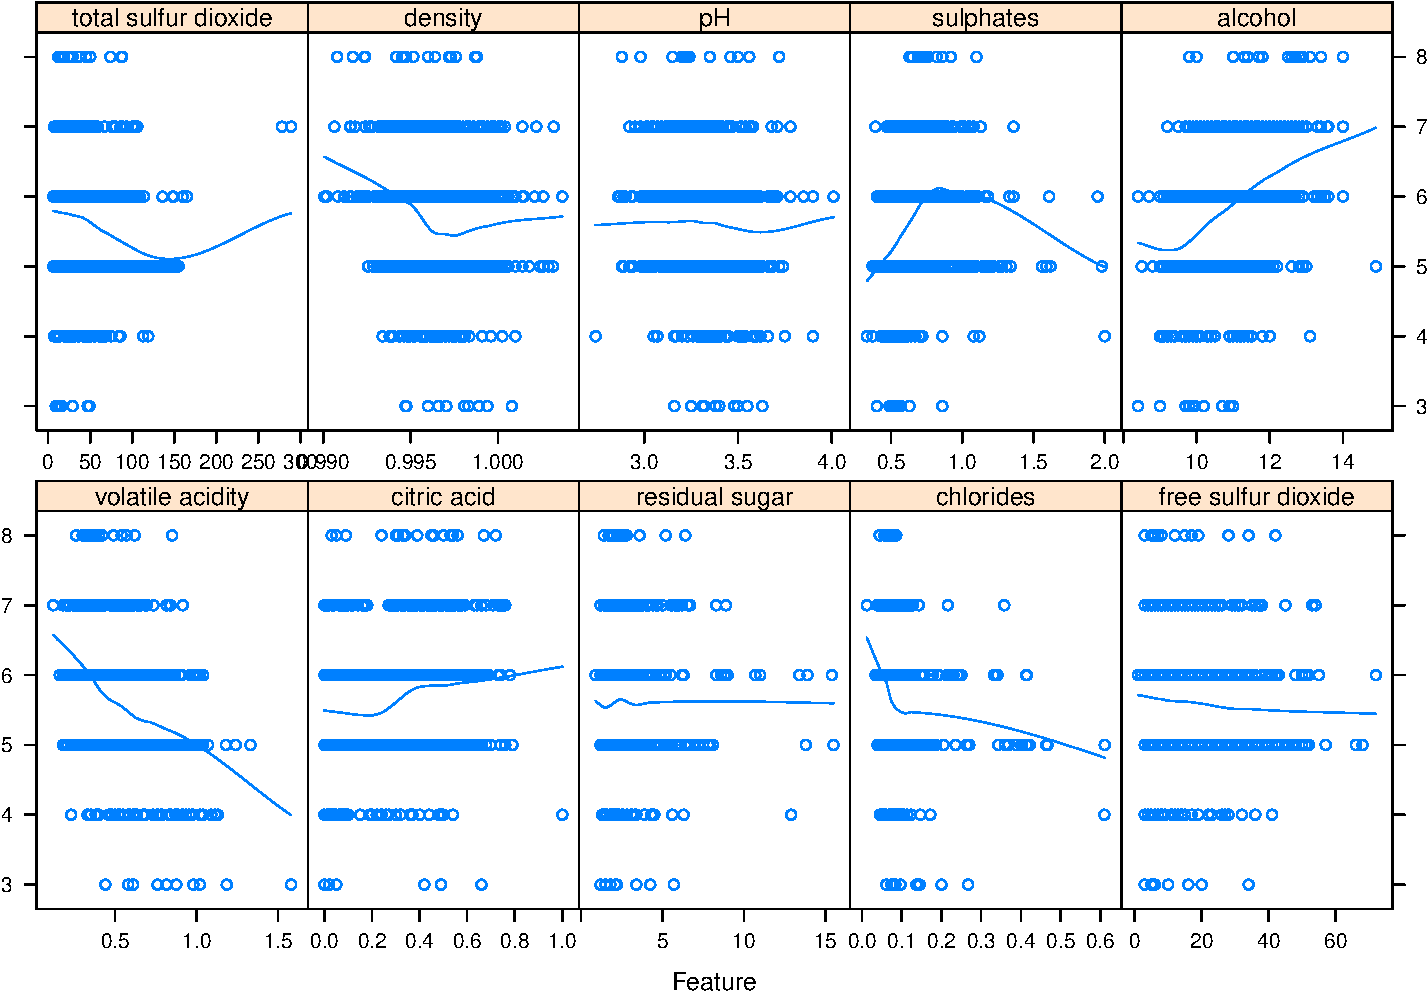
\includegraphics{ML_with_caret_files/figure-beamer/unnamed-chunk-1-1.pdf}

\end{frame}

\begin{frame}[fragile]{Define Class Variable}

\begin{Shaded}
\begin{Highlighting}[]
\NormalTok{quality.wine.df =}\StringTok{ }\NormalTok{wine.df }\OperatorTok\StringTok{ }\KeywordTok{mutate}\NormalTok{(}\DataTypeTok{goodwine =} \KeywordTok{if_else}\NormalTok{(quality}\OperatorTok{>}\DecValTok{5}\NormalTok{, }\StringTok{"good"}\NormalTok{, }\StringTok{"bad"}\NormalTok{)) }\OperatorTok\StringTok{ }
\StringTok{  }\KeywordTok{mutate}\NormalTok{(}\DataTypeTok{goodwine =} \KeywordTok{as.factor}\NormalTok{(goodwine))}

\KeywordTok{ggplot}\NormalTok{(quality.wine.df, }\KeywordTok{aes}\NormalTok{(goodwine, quality, }\DataTypeTok{colour =}\NormalTok{ goodwine, }\DataTypeTok{fill =}\NormalTok{ goodwine))}\OperatorTok{+}
\StringTok{  }\KeywordTok{geom_point}\NormalTok{(}\DataTypeTok{size =}\NormalTok{ .}\DecValTok{5}\NormalTok{, }\DataTypeTok{alpha =}\NormalTok{ .}\DecValTok{7}\NormalTok{, }\DataTypeTok{position =} \KeywordTok{position_jitter}\NormalTok{(}\DataTypeTok{height =} \FloatTok{0.1}\NormalTok{))}\OperatorTok{+}
\StringTok{  }\KeywordTok{labs}\NormalTok{(}\DataTypeTok{x =} \StringTok{"Discretized wine quality"}\NormalTok{, }\DataTypeTok{y =} \StringTok{"Rated wine quality"}\NormalTok{)}\OperatorTok{+}
\StringTok{  }\KeywordTok{theme}\NormalTok{(}\DataTypeTok{legend.position =} \StringTok{"none"}\NormalTok{)}
\end{Highlighting}
\end{Shaded}

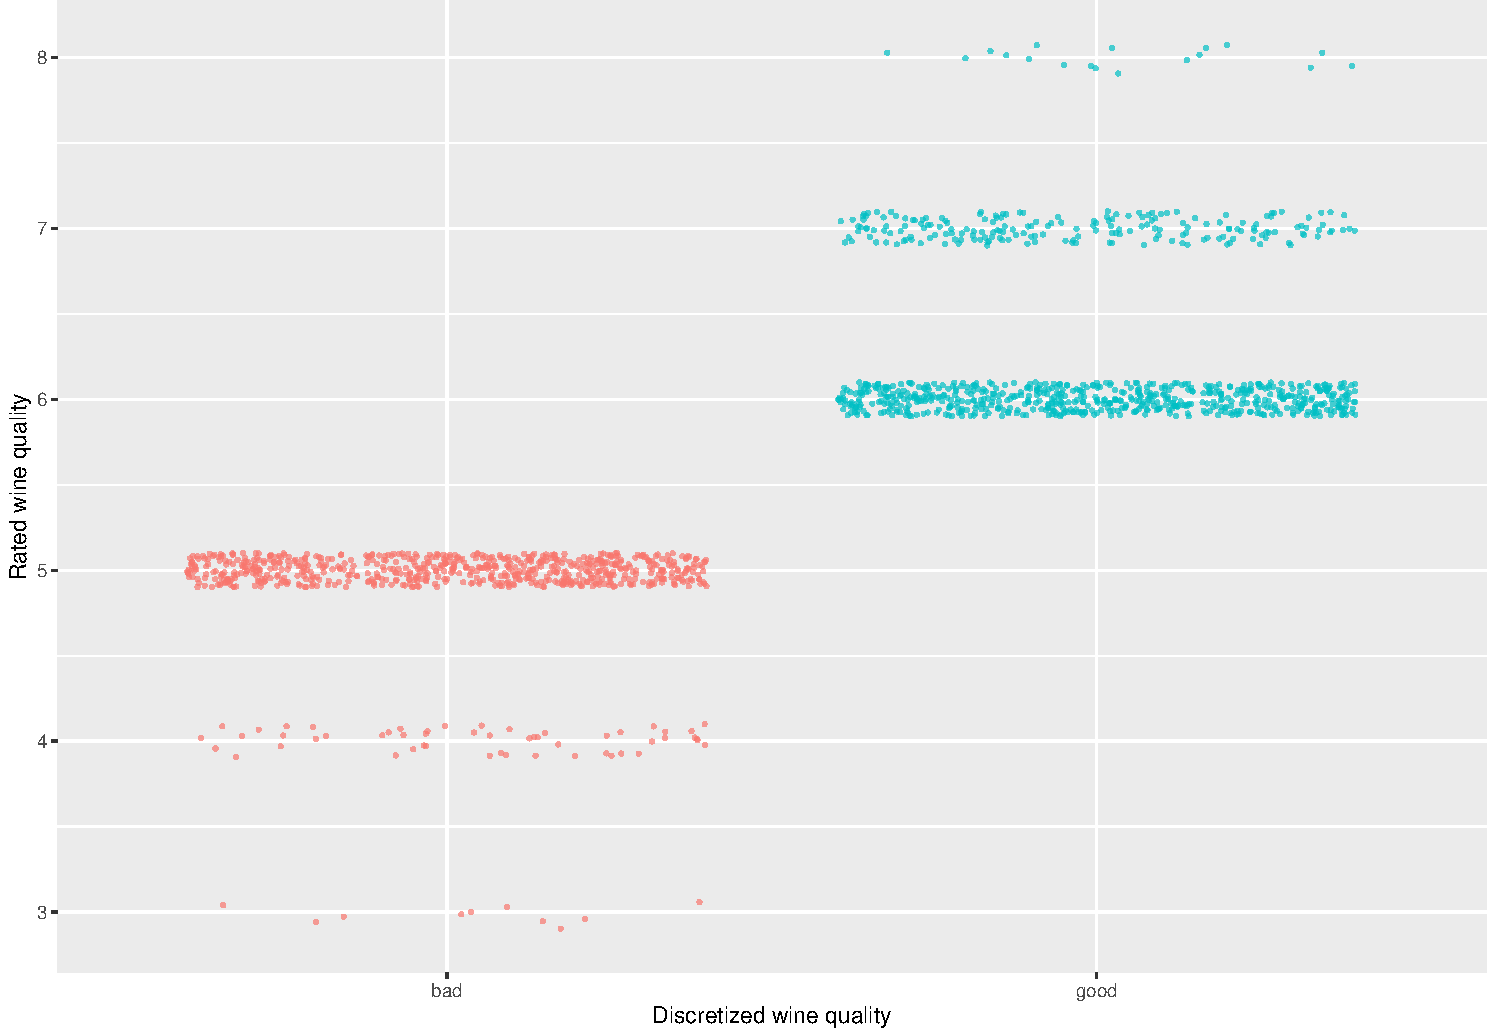
\includegraphics[width=0.6\linewidth]{ML_with_caret_files/figure-beamer/define-class-1}

\begin{Shaded}
\begin{Highlighting}[]
\NormalTok{wine.df =}\StringTok{ }\NormalTok{quality.wine.df }\OperatorTok\StringTok{ }\KeywordTok{select}\NormalTok{(}\OperatorTok{-}\NormalTok{quality)}
\end{Highlighting}
\end{Shaded}

\end{frame}

\begin{frame}{Holdout Validation}

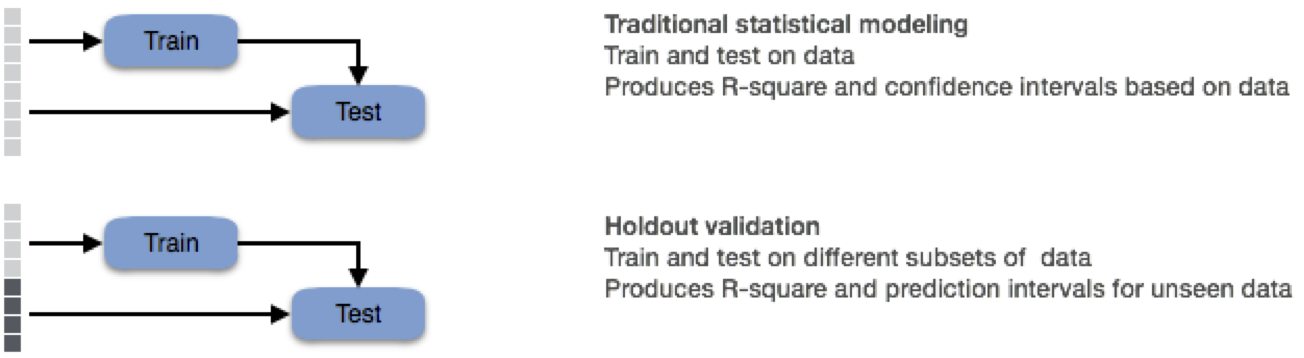
\includegraphics[width=10.87in]{1.FittingValidation}

\end{frame}

\begin{frame}{Cross-validation: Repeated k-fold cross-validation}

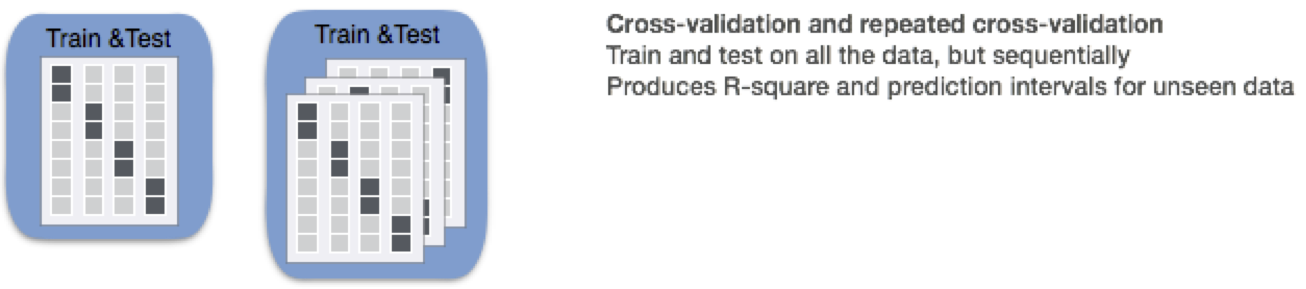
\includegraphics[width=10.88in]{2. CrossvalidationRepeatedcrossvalidation}

\end{frame}

\begin{frame}{Cross-validation: Hyperparameter tuning}

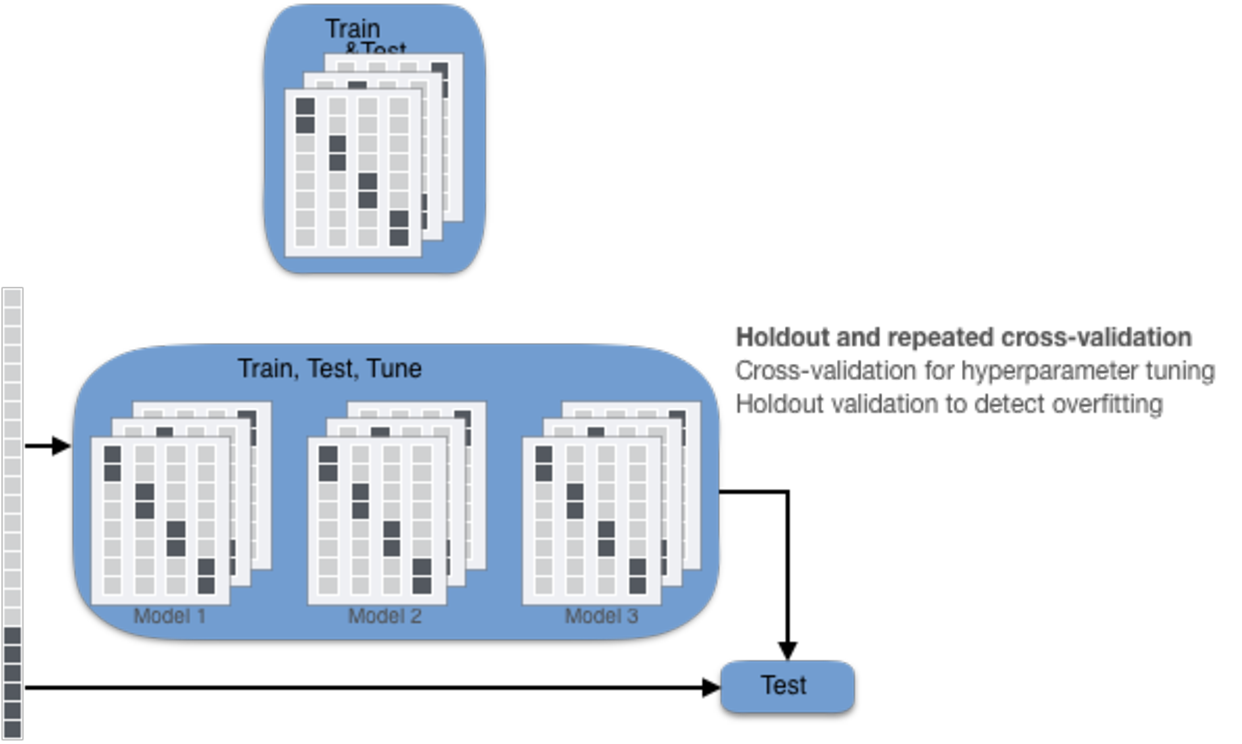
\includegraphics[width=4.97in]{3.TrainTestTune}

\end{frame}

\begin{frame}[fragile]{Partition Data into Training and Testing}

-- Proportions of class variable---good and bad wine---should be similar

-- Proportions of class variables should be similar in test and training
data

-- \texttt{createDataPartition} Creates partitions that maintains the
class distribution

\end{frame}

\begin{frame}[fragile]{Partition Data into Training and Testing}

\begin{Shaded}
\begin{Highlighting}[]
\NormalTok{inTrain =}\StringTok{ }\KeywordTok{createDataPartition}\NormalTok{(wine.df}\OperatorTok{$}\NormalTok{goodwine, }\DataTypeTok{p =} \DecValTok{3}\OperatorTok{/}\DecValTok{4}\NormalTok{, }\DataTypeTok{list =} \OtherTok{FALSE}\NormalTok{)}

\NormalTok{trainDescr =}\StringTok{ }\NormalTok{wine.df[inTrain, }\OperatorTok{-}\DecValTok{12}\NormalTok{] }\CommentTok{# All but class variable}
\NormalTok{testDescr =}\StringTok{ }\NormalTok{wine.df[}\OperatorTok{-}\NormalTok{inTrain, }\OperatorTok{-}\DecValTok{12}\NormalTok{]}

\NormalTok{trainClass =}\StringTok{ }\NormalTok{wine.df}\OperatorTok{$}\NormalTok{goodwine[inTrain] }
\NormalTok{testClass =}\StringTok{ }\NormalTok{wine.df}\OperatorTok{$}\NormalTok{goodwine[}\OperatorTok{-}\NormalTok{inTrain]}
\end{Highlighting}
\end{Shaded}

\end{frame}

\begin{frame}[fragile]{Partition Data into Training and Testing}

\begin{Shaded}
\begin{Highlighting}[]
\NormalTok{wine.df}\OperatorTok{$}\NormalTok{goodwine }\OperatorTok\StringTok{  }\KeywordTok{table}\NormalTok{() }\OperatorTok\StringTok{ }\KeywordTok{prop.table}\NormalTok{() }\OperatorTok\StringTok{ }\KeywordTok{round}\NormalTok{(}\DecValTok{3}\NormalTok{)}\OperatorTok{*}\DecValTok{100} 
\end{Highlighting}
\end{Shaded}

\begin{verbatim}
## .
##  bad good 
## 46.5 53.5
\end{verbatim}

\begin{Shaded}
\begin{Highlighting}[]
\NormalTok{trainClass }\OperatorTok\StringTok{ }\KeywordTok{table}\NormalTok{() }\OperatorTok\StringTok{ }\KeywordTok{prop.table}\NormalTok{() }\OperatorTok\StringTok{ }\KeywordTok{round}\NormalTok{(}\DecValTok{3}\NormalTok{)}\OperatorTok{*}\DecValTok{100}
\end{Highlighting}
\end{Shaded}

\begin{verbatim}
## .
##  bad good 
## 46.5 53.5
\end{verbatim}

\begin{Shaded}
\begin{Highlighting}[]
\NormalTok{testClass }\OperatorTok\StringTok{ }\KeywordTok{table}\NormalTok{() }\OperatorTok\StringTok{ }\KeywordTok{prop.table}\NormalTok{() }\OperatorTok\StringTok{ }\KeywordTok{round}\NormalTok{(}\DecValTok{3}\NormalTok{)}\OperatorTok{*}\DecValTok{100}
\end{Highlighting}
\end{Shaded}

\begin{verbatim}
## .
##  bad good 
## 46.6 53.4
\end{verbatim}

\end{frame}

\begin{frame}{Pre-process Data: Filter poor predictors}

-- Eliminate variables with no variabilty

-- Eliminate highly correlated variables

-- Select predictive features

-- Engineer predictive features

\end{frame}

\begin{frame}[fragile]{Pre-process Data: Normalization}

-- \texttt{preProcess} also supports other preprocessing methods, such
as PCA and ICA

-- \texttt{center} subtracts mean

-- \texttt{scale} normalizes based on standard deviation

\begin{Shaded}
\begin{Highlighting}[]
\NormalTok{xTrans =}\StringTok{ }\KeywordTok{preProcess}\NormalTok{(trainDescr, }\DataTypeTok{method =} \KeywordTok{c}\NormalTok{(}\StringTok{"center"}\NormalTok{, }\StringTok{"scale"}\NormalTok{)) }
\NormalTok{trainScaled =}\StringTok{ }\KeywordTok{predict}\NormalTok{(xTrans, trainDescr)}
\NormalTok{testScaled =}\StringTok{ }\KeywordTok{predict}\NormalTok{(xTrans, testDescr)}
\end{Highlighting}
\end{Shaded}

\end{frame}

\begin{frame}{Pre-process Data: Normalization}

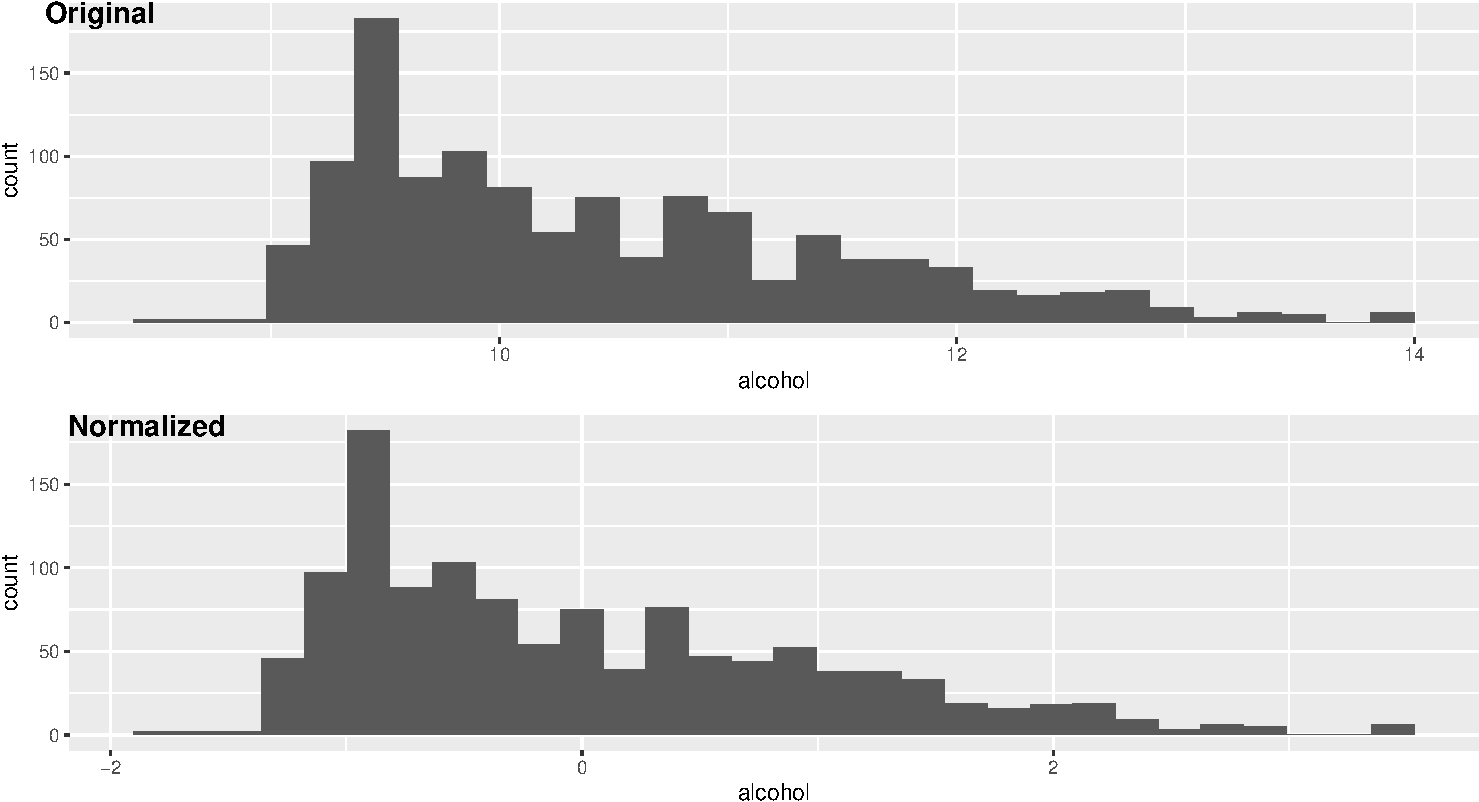
\includegraphics{ML_with_caret_files/figure-beamer/pre-process-plot-1.pdf}

\end{frame}

\begin{frame}[fragile]{Exercise: Partition and pre-process data}

-- Load and review the Wisconsin cancer data

\texttt{cancer.df\ =\ read\_csv("cancer.csv")}

\texttt{skim(cancer.df)}

-- Identify the diagnosis indicator

-- Partition data

\texttt{inTrain\ =\ createDataPartition(cancer.df\$diagnosis,\ p\ =\ 3/4,\ list\ =\ FALSE)}

\texttt{trainDescr\ =\ cancer.df{[}inTrain,\ -(1:2){]}\ \#\ All\ but\ class\ variable}

\texttt{testDescr\ =\ cancer.df{[}-inTrain,\ -(1:2){]}}

\texttt{trainClass\ =\ cancer.df\$diagnosis{[}inTrain{]}}

\texttt{testClass\ =\ cancer.df\$diagnosis{[}-inTrain{]}}

-- Pre-process data

\texttt{xTrans\ =\ preProcess(trainDescr,\ method\ =\ c("center",\ "scale"))}

\texttt{trainScaled\ =\ predict(xTrans,\ trainDescr)}

\texttt{testScaled\ =\ predict(xTrans,\ testDescr)}

\end{frame}

\begin{frame}{Cross Validation}

-- Used to select best combination of predictors and model parameters

-- Estimates model performance (e.g., AUC or r-square) for each
candidate model

-- Uses a random subset of the training data to train the model and a
withheld subset to test

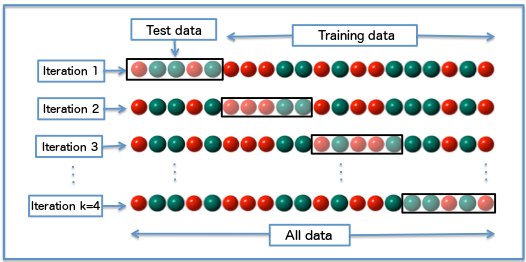
\includegraphics[width=7.01in]{K-fold_cross_validation}

\end{frame}

\begin{frame}[fragile]{Grouped Cross-validation\textbar{}Sleep study
example}

\texttt{sleep.df\ =\ sleepstudy}
\texttt{folds\ \textless{}-\ groupKFold(sleep.df\$Subject,\ k\ =\ 18)}

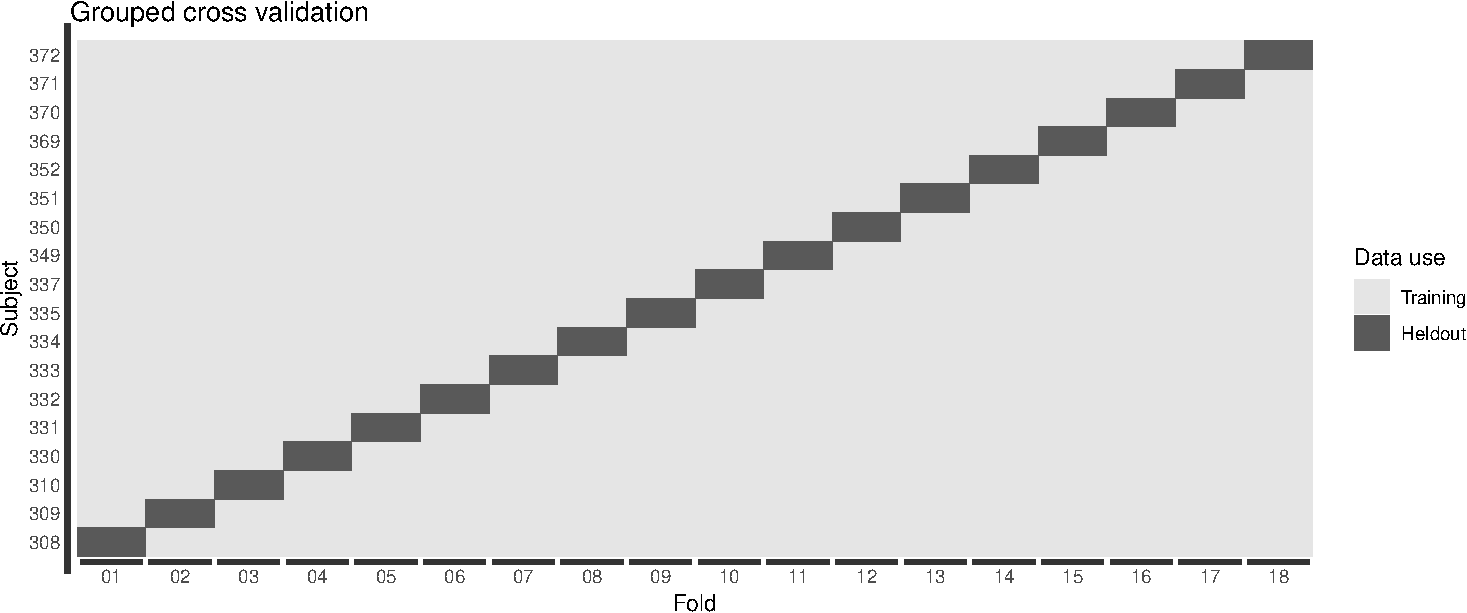
\includegraphics{ML_with_caret_files/figure-beamer/groupfold-1.pdf}

\end{frame}

\begin{frame}[fragile]{Define Training Parameters}

-- Select cross validation method: 10-fold repeated cross validation is
common

-- Define hyperparameter selection method: grid search is the simplest
approach

-- Define summary measures

-- \texttt{trainControl} command specifies all these parameters in a
single statement

\end{frame}

\begin{frame}[fragile]{Define Training Parameters:
\texttt{trainControl}}

\begin{Shaded}
\begin{Highlighting}[]
\NormalTok{train.control =}\StringTok{ }\KeywordTok{trainControl}\NormalTok{(}\DataTypeTok{method =} \StringTok{"repeatedcv"}\NormalTok{, }
                              \DataTypeTok{number =} \DecValTok{10}\NormalTok{, }\DataTypeTok{repeats =} \DecValTok{3}\NormalTok{, }\CommentTok{# number: number of folds}
                              \DataTypeTok{search =} \StringTok{"grid"}\NormalTok{, }\CommentTok{# for tuning hyperparameters}
                              \DataTypeTok{classProbs =} \OtherTok{TRUE}\NormalTok{,}
                              \DataTypeTok{savePredictions =} \StringTok{"final"}\NormalTok{,}
                              \DataTypeTok{summaryFunction =}\NormalTok{ twoClassSummary)}
\end{Highlighting}
\end{Shaded}

\end{frame}

\begin{frame}[fragile]{Select Models to Train}

-- Over 200 different models from 50 categories (e.g., Linear
regression, boosting, bagging, cost sensitive learning)

-- List of models:
\url{http://caret.r-forge.r-project.org/modelList.html}

-- The ``train'' statement can train any of them

-- Here we select three:

\begin{verbatim}
- Logistic regression

- Support vector machine

- Xgboost, a boosted random forest that performs well in many situations
\end{verbatim}

\end{frame}

\begin{frame}{Train Models and Tune Hyperparameters with the
\texttt{train} function}

-- Specify class and predictor variables

-- Specify one of the over 200 models (e.g., xgboost)

-- Specify the metric, such as ROC

-- Include the train control specified earlier

\end{frame}

\begin{frame}{Train Models and Tune Hyperparameters: Logistic
regression}

-- Logistic regression has no tuning parameters

-- 10-fold repeated (3 times) cross-validation occurs once

-- Produces a total of 30 instances of model fitting and testing

-- Cross validation provides a nearly unbiased estimate of the
performance of the model on the held out data

\end{frame}

\begin{frame}[fragile]{Train Models and Tune Hyperparameters: Logistic
regression}

\begin{Shaded}
\begin{Highlighting}[]
\NormalTok{glm.fit =}\StringTok{ }\KeywordTok{train}\NormalTok{(}\DataTypeTok{x =}\NormalTok{ trainScaled, }\DataTypeTok{y =}\NormalTok{ trainClass,}
   \DataTypeTok{method =} \StringTok{'glm'}\NormalTok{, }\DataTypeTok{metric =} \StringTok{"ROC"}\NormalTok{,}
   \DataTypeTok{trControl =}\NormalTok{ train.control) }

\NormalTok{glm.fit}
\end{Highlighting}
\end{Shaded}

\begin{verbatim}
## Generalized Linear Model 
## 
## 1200 samples
##   11 predictor
##    2 classes: 'bad', 'good' 
## 
## No pre-processing
## Resampling: Cross-Validated (10 fold, repeated 3 times) 
## Summary of sample sizes: 1079, 1080, 1080, 1080, 1080, 1080, ... 
## Resampling results:
## 
##   ROC        Sens       Spec     
##   0.8083925  0.7282143  0.7502404
\end{verbatim}

\end{frame}

\begin{frame}{Train Models and Tune Hyperparameters: Support vector
machine}

\begin{itemize}
\item
  Linear support vector machines have a single tuning parameter--C
\item
  C (Cost)
\item
  C = 1000 ``hard margin'' tends to be sensitive to individual data
  points and is prone to over fitting
\end{itemize}

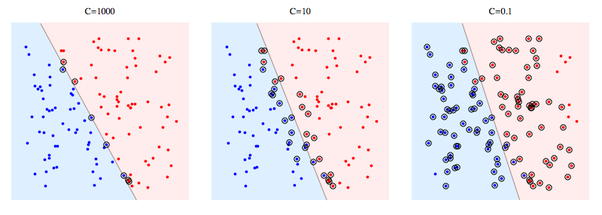
\includegraphics[width=0.85\linewidth]{SVM-Cparameter}

\url{https://stackoverflow.com/questions/4629505/svm-hard-or-soft-margins}

\end{frame}

\begin{frame}[fragile]{Train Models and Tune Hyperparameters: Support
vector machine}

\begin{Shaded}
\begin{Highlighting}[]
\NormalTok{grid =}\StringTok{ }\KeywordTok{expand.grid}\NormalTok{(}\DataTypeTok{C =} \KeywordTok{c}\NormalTok{(.}\DecValTok{1}\NormalTok{, .}\DecValTok{2}\NormalTok{, .}\DecValTok{4}\NormalTok{, }\DecValTok{1}\NormalTok{, }\DecValTok{2}\NormalTok{, }\DecValTok{4}\NormalTok{))}
\NormalTok{svm.fit =}\StringTok{  }\KeywordTok{train}\NormalTok{(}\DataTypeTok{x =}\NormalTok{ trainScaled, }\DataTypeTok{y =}\NormalTok{ trainClass,}
  \DataTypeTok{method =} \StringTok{"svmLinear"}\NormalTok{, }\DataTypeTok{metric =} \StringTok{"ROC"}\NormalTok{,}
  \DataTypeTok{tuneGrid =}\NormalTok{ grid, }\CommentTok{# Overrides tuneLength}
  \DataTypeTok{tuneLength =} \DecValTok{3}\NormalTok{, }\CommentTok{# Number of levels of each hyper parameter, unless specified by grid}
  \DataTypeTok{trControl =}\NormalTok{ train.control, }\DataTypeTok{scaled =} \OtherTok{TRUE}\NormalTok{)}

\KeywordTok{plot}\NormalTok{(svm.fit)}
\end{Highlighting}
\end{Shaded}

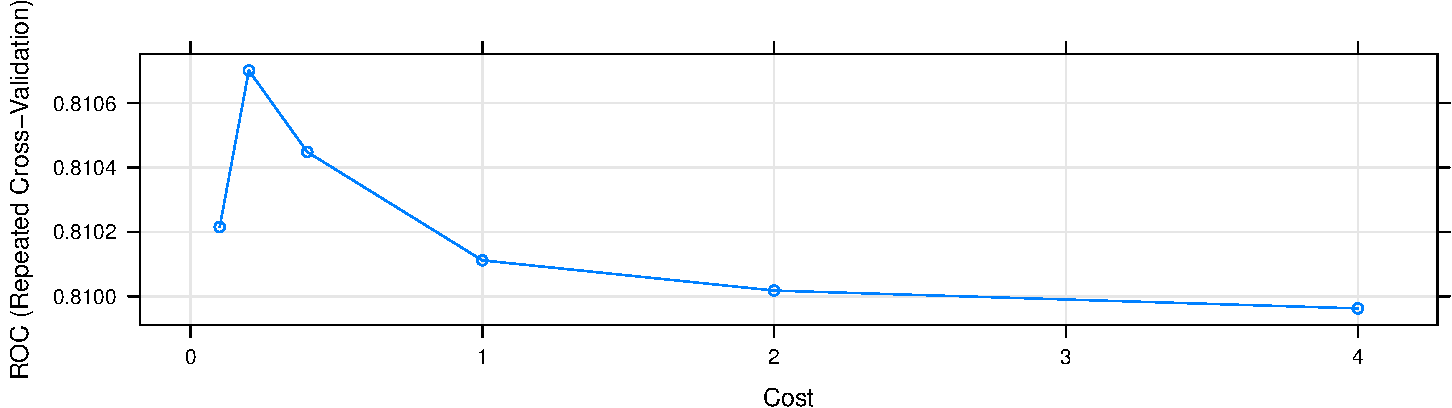
\includegraphics{ML_with_caret_files/figure-beamer/train_svm-1.pdf}

\end{frame}

\begin{frame}{Train Models and Tune Hyperparameters: xgboost}

Classification depends on adding outcomes across many trees

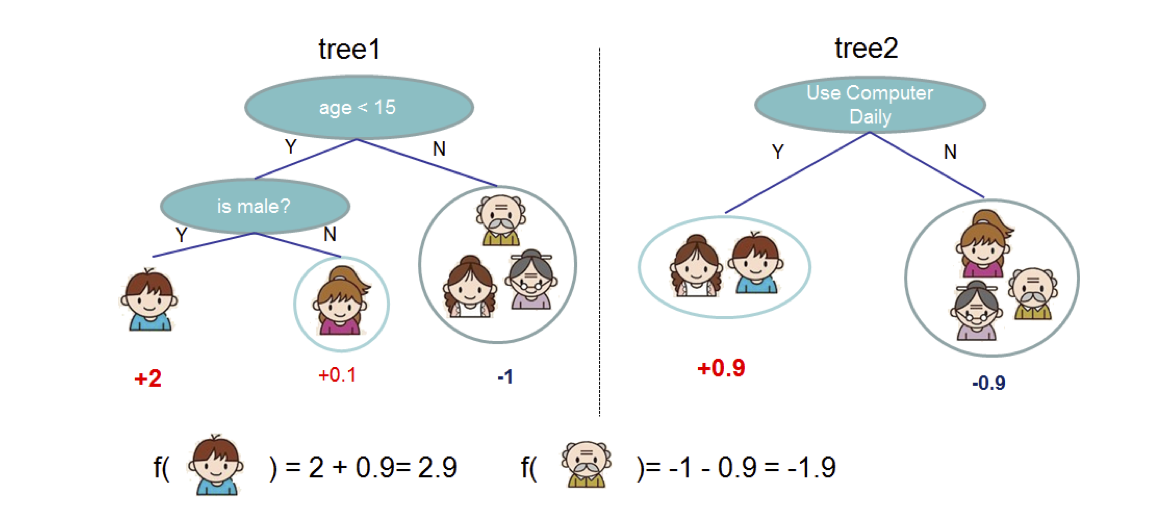
\includegraphics[width=0.85\linewidth]{xgboost_trees}

{Chen, T., \& Guestrin, C. (2016). XGBoost: A scalable tree boosting
system. Proceedings of the 22nd ACM SIGKDD International Conference on
Knowledge Discovery and Data Mining, 785--794.}

\end{frame}

\begin{frame}{Train Models and Tune Hyperparameters: xgboost}

Trees are built in sequence to address the errors (residuals) of the
previous trees

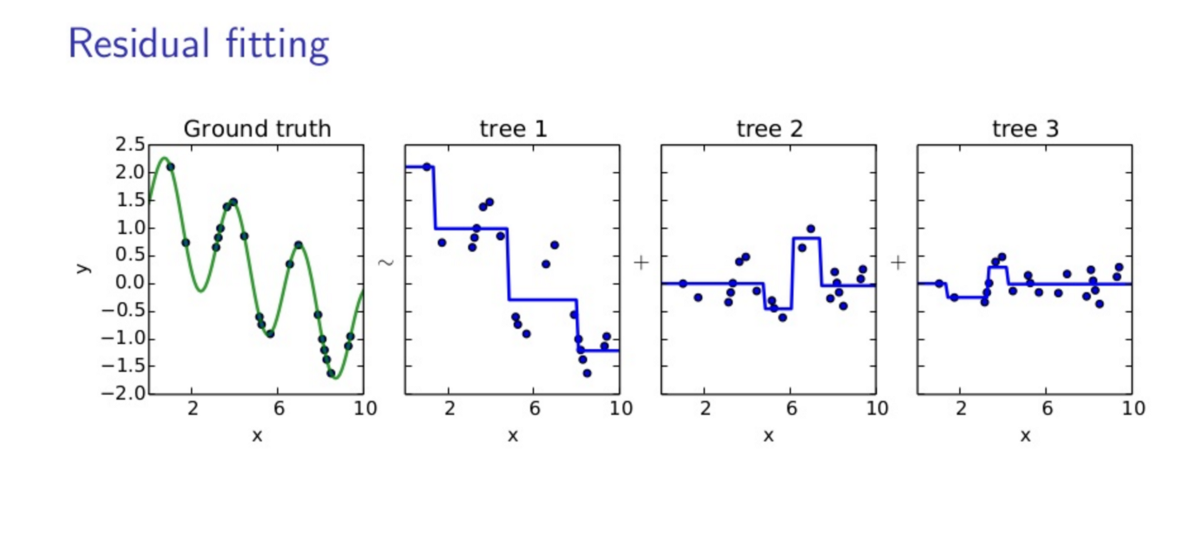
\includegraphics[width=0.9\linewidth]{xgboost_residualfitting}

{\url{https://towardsdatascience.com/}}

\end{frame}

\begin{frame}{Train Models and Tune Hyperparameters: xgboost}

-- nrounds (\# Boosting Iterations)--model robustness

-- max\_depth (Max Tree Depth)--model complexity

-- eta (Shrinkage)--model robustness

-- gamma (Minimum Loss Reduction)--model complexity

-- colsample\_bytree (Subsample Ratio of Columns)--model robustness

-- min\_child\_weight (Minimum Sum of Instance Weight)--model complexity

-- subsample (Subsample Percentage)--model robustness

\textbf{A grid search with 3 levels for each parameter produces 3\^{}7
combinations!}

\end{frame}

\begin{frame}[fragile]{Train Models and Tune Hyperparameters: xgboost}

\texttt{tuneLength\ =\ 3} produces

\begin{verbatim}
- nrounds (# Boosting Iterations) (50 100 150)

- max_depth (Max Tree Depth) (1, 2, 3)

- eta (Shrinkage) (.3, .4)

- gamma (Minimum Loss Reduction) (0)

- colsample_bytree (Subsample Ratio of Columns) (.6, .8)

- min_child_weight (Minimum Sum of Instance Weight) (1)

- subsample (Subsample Percentage) (.50, .75, 1.0)
\end{verbatim}

-- 108 different model combinations each trained and tested 10X3 times

\end{frame}

\begin{frame}[fragile]{Train models and tune Hyperparameters: xgboost}

\begin{Shaded}
\begin{Highlighting}[]
\NormalTok{xgb.fit =}\StringTok{ }\KeywordTok{train}\NormalTok{(}\DataTypeTok{x =}\NormalTok{ trainScaled, }\DataTypeTok{y =}\NormalTok{ trainClass,}
  \DataTypeTok{method =} \StringTok{"xgbTree"}\NormalTok{, }\DataTypeTok{metric =} \StringTok{"ROC"}\NormalTok{,}
  \DataTypeTok{tuneLength =} \DecValTok{3}\NormalTok{, }\CommentTok{# Depends on number of parameters in algorithm}
  \DataTypeTok{trControl =}\NormalTok{ train.control, }\DataTypeTok{scaled =} \OtherTok{TRUE}\NormalTok{)}
\end{Highlighting}
\end{Shaded}

\end{frame}

\begin{frame}{Train models and tune: xgboost}

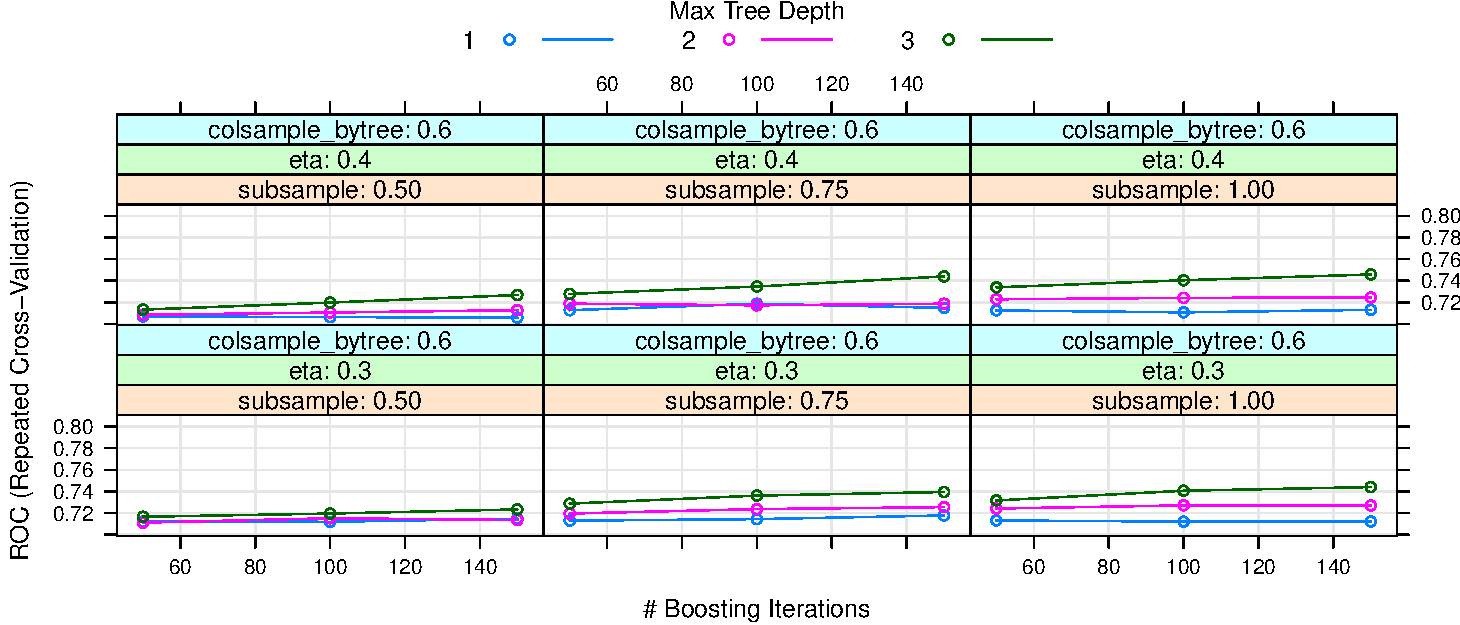
\includegraphics{ML_with_caret_files/figure-beamer/plot_train_xgb-1.pdf}
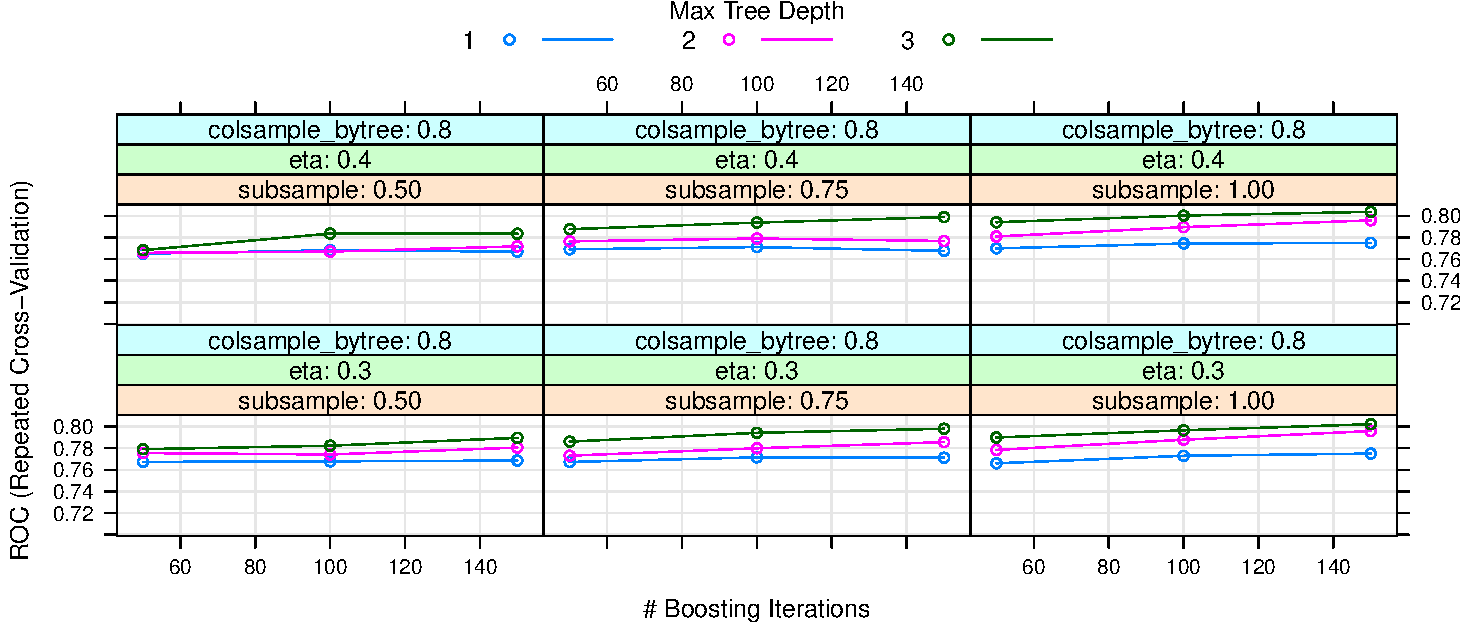
\includegraphics{ML_with_caret_files/figure-beamer/plot_train_xgb-2.pdf}

\end{frame}

\begin{frame}[fragile]{Exercise: Train and Tune Hyperparameters}

-- Set training parameters

\texttt{train.control\ =} \texttt{trainControl(method\ =\ "repeatedcv",}
\texttt{number\ =\ 10,\ repeats\ =\ 3,\ \#\ number:\ number\ of\ folds}
\texttt{search\ =\ "grid",\ \#\ for\ tuning\ hyperparameters}
\texttt{classProbs\ =\ TRUE,} \texttt{savePredictions\ =\ "final",}
\texttt{summaryFunction\ =\ twoClassSummary)}

-- Train an extreme boosting tree

\texttt{xgb.fit\ =\ train(x\ =\ trainScaled,\ y\ =\ trainClass,}
\texttt{method\ =\ "xgbTree",\ metric\ =\ "ROC",}
\texttt{tuneLength\ =\ 3,\ \#\ Depends\ on\ number\ of\ parameters\ in\ algorithm}
\texttt{trControl\ =\ train.control,\ scaled\ =\ TRUE)}

-- Identify the best combination of Hyperparameters

\end{frame}

\begin{frame}[fragile]{Assess Performance: Confusion matrix (glm)}

\begin{Shaded}
\begin{Highlighting}[]
\NormalTok{glm.pred =}\StringTok{ }\KeywordTok{predict}\NormalTok{(glm.fit, testScaled)}

\KeywordTok{confusionMatrix}\NormalTok{(glm.pred, testClass)}
\end{Highlighting}
\end{Shaded}

\begin{verbatim}
## Confusion Matrix and Statistics
## 
##           Reference
## Prediction bad good
##       bad  142   54
##       good  44  159
##                                           
##                Accuracy : 0.7544          
##                  95% CI : (0.7091, 0.7959)
##     No Information Rate : 0.5338          
##     P-Value [Acc > NIR] : <2e-16          
##                                           
##                   Kappa : 0.5082          
##  Mcnemar's Test P-Value : 0.3633          
##                                           
##             Sensitivity : 0.7634          
##             Specificity : 0.7465          
##          Pos Pred Value : 0.7245          
##          Neg Pred Value : 0.7833          
##              Prevalence : 0.4662          
##          Detection Rate : 0.3559          
##    Detection Prevalence : 0.4912          
##       Balanced Accuracy : 0.7550          
##                                           
##        'Positive' Class : bad             
## 
\end{verbatim}

\end{frame}

\begin{frame}[fragile]{Assess Performance: Confusion matrix (svm)}

\begin{Shaded}
\begin{Highlighting}[]
\NormalTok{svm.pred =}\StringTok{ }\KeywordTok{predict}\NormalTok{(svm.fit, testScaled)}

\KeywordTok{confusionMatrix}\NormalTok{(svm.pred, testClass)}
\end{Highlighting}
\end{Shaded}

\begin{verbatim}
## Confusion Matrix and Statistics
## 
##           Reference
## Prediction bad good
##       bad  146   58
##       good  40  155
##                                           
##                Accuracy : 0.7544          
##                  95% CI : (0.7091, 0.7959)
##     No Information Rate : 0.5338          
##     P-Value [Acc > NIR] : < 2e-16         
##                                           
##                   Kappa : 0.5095          
##  Mcnemar's Test P-Value : 0.08593         
##                                           
##             Sensitivity : 0.7849          
##             Specificity : 0.7277          
##          Pos Pred Value : 0.7157          
##          Neg Pred Value : 0.7949          
##              Prevalence : 0.4662          
##          Detection Rate : 0.3659          
##    Detection Prevalence : 0.5113          
##       Balanced Accuracy : 0.7563          
##                                           
##        'Positive' Class : bad             
## 
\end{verbatim}

\end{frame}

\begin{frame}[fragile]{Assess Performance: Confusion matrix (xgb)}

\begin{Shaded}
\begin{Highlighting}[]
\NormalTok{xgb.pred =}\StringTok{ }\KeywordTok{predict}\NormalTok{(xgb.fit, testScaled)}

\KeywordTok{confusionMatrix}\NormalTok{(xgb.pred, testClass)}
\end{Highlighting}
\end{Shaded}

\begin{verbatim}
## Confusion Matrix and Statistics
## 
##           Reference
## Prediction bad good
##       bad  166   19
##       good  20  194
##                                           
##                Accuracy : 0.9023          
##                  95% CI : (0.8688, 0.9296)
##     No Information Rate : 0.5338          
##     P-Value [Acc > NIR] : <2e-16          
##                                           
##                   Kappa : 0.8035          
##  Mcnemar's Test P-Value : 1               
##                                           
##             Sensitivity : 0.8925          
##             Specificity : 0.9108          
##          Pos Pred Value : 0.8973          
##          Neg Pred Value : 0.9065          
##              Prevalence : 0.4662          
##          Detection Rate : 0.4160          
##    Detection Prevalence : 0.4637          
##       Balanced Accuracy : 0.9016          
##                                           
##        'Positive' Class : bad             
## 
\end{verbatim}

\end{frame}

\begin{frame}[fragile]{Compare Models}

\begin{Shaded}
\begin{Highlighting}[]
\NormalTok{mod.resamps =}\StringTok{ }\KeywordTok{resamples}\NormalTok{(}\KeywordTok{list}\NormalTok{(}\DataTypeTok{glm =}\NormalTok{ glm.fit, }\DataTypeTok{svm =}\NormalTok{ svm.fit, }\DataTypeTok{xgb =}\NormalTok{ xgb.fit))}

\KeywordTok{bwplot}\NormalTok{(mod.resamps, }\DataTypeTok{metric=}\StringTok{"ROC"}\NormalTok{)}
\end{Highlighting}
\end{Shaded}

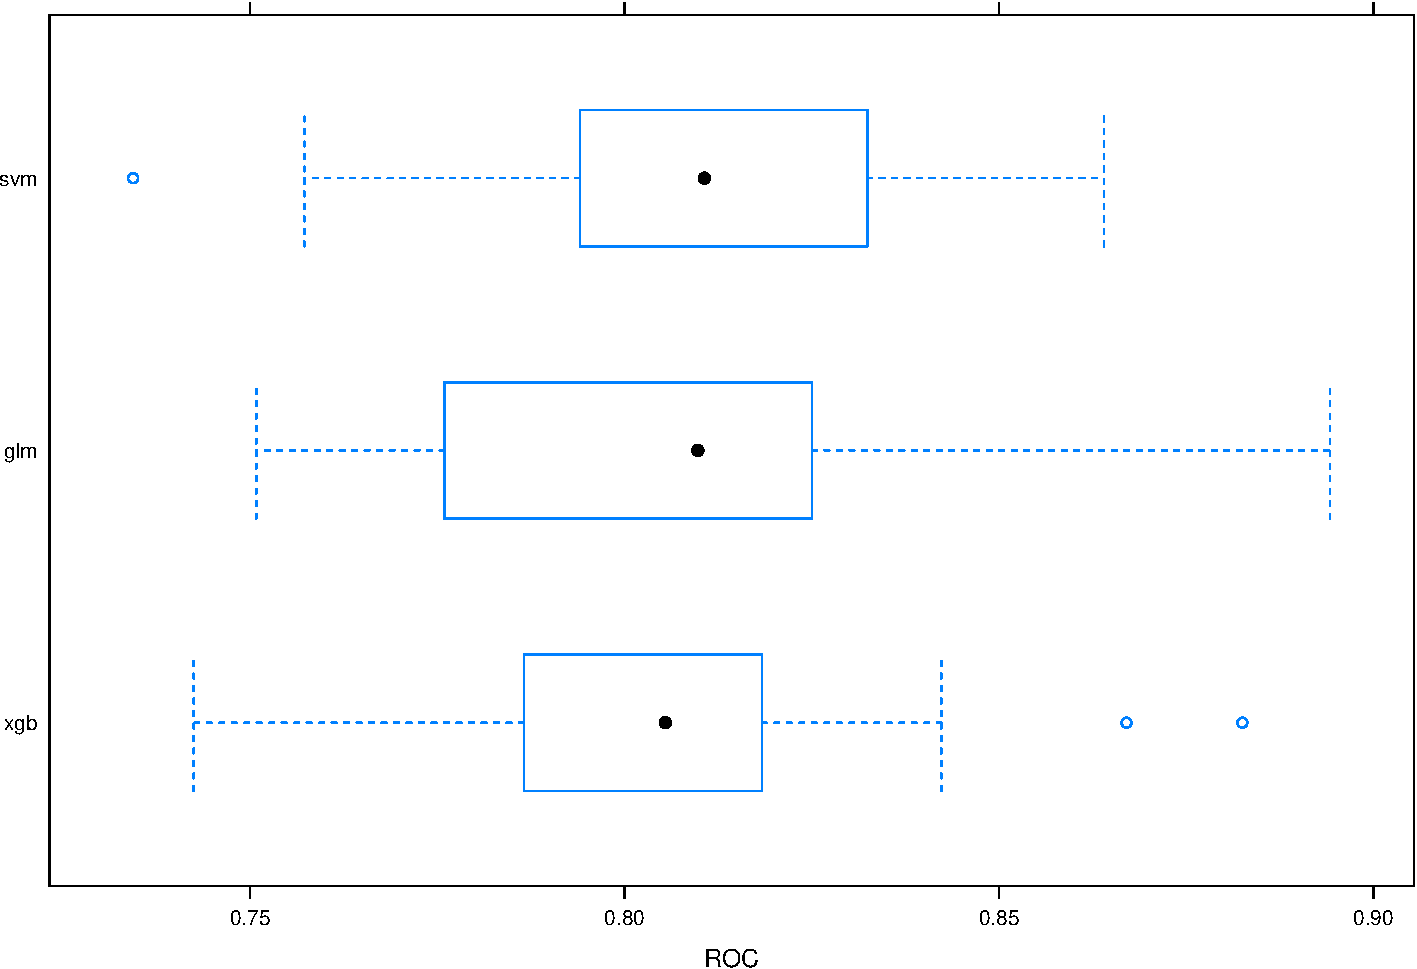
\includegraphics{ML_with_caret_files/figure-beamer/compare_boxplot-1.pdf}

\begin{Shaded}
\begin{Highlighting}[]
\CommentTok{# dotplot(mod.resamps, metric="ROC")}
\end{Highlighting}
\end{Shaded}

\end{frame}

\begin{frame}{Assess Performance (xgb): ROC plot}

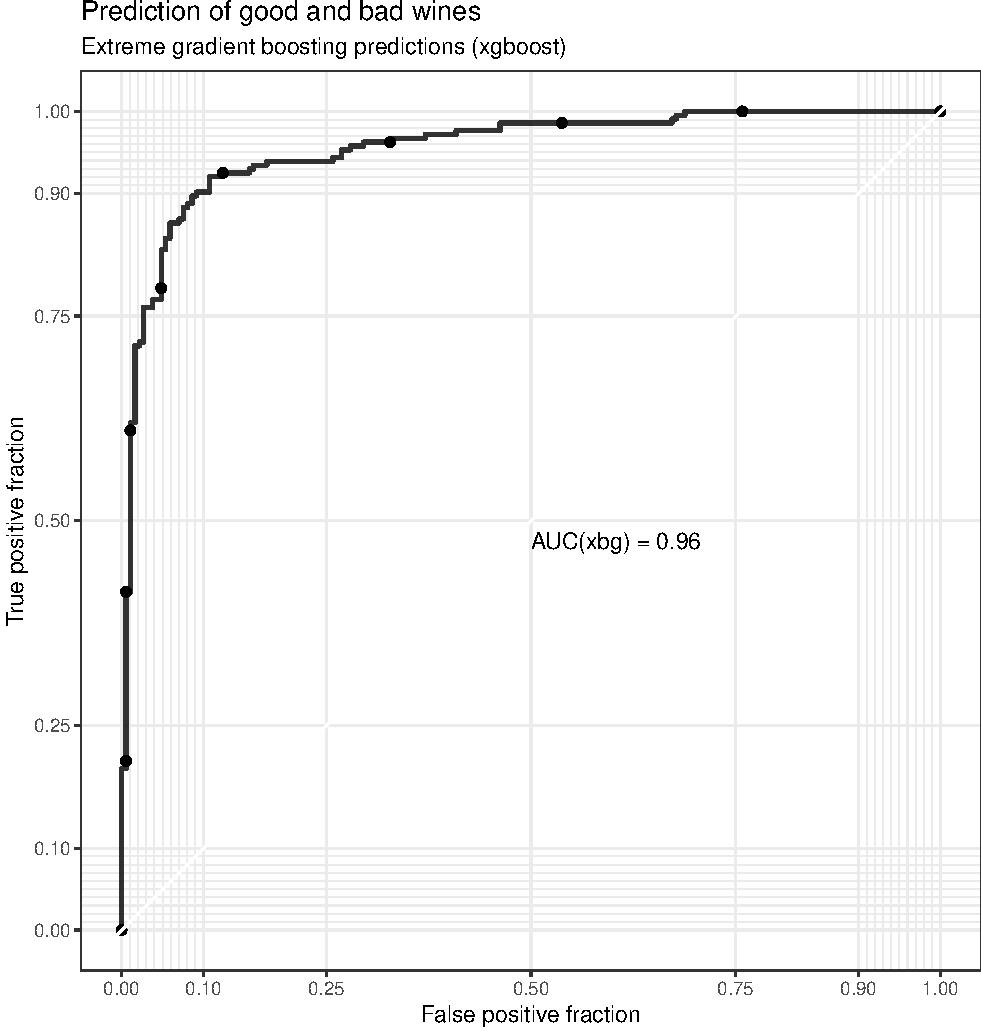
\includegraphics[width=0.9\linewidth]{ML_with_caret_files/figure-beamer/assess_ROC-1}

\end{frame}

\begin{frame}{xgboost Predictions}

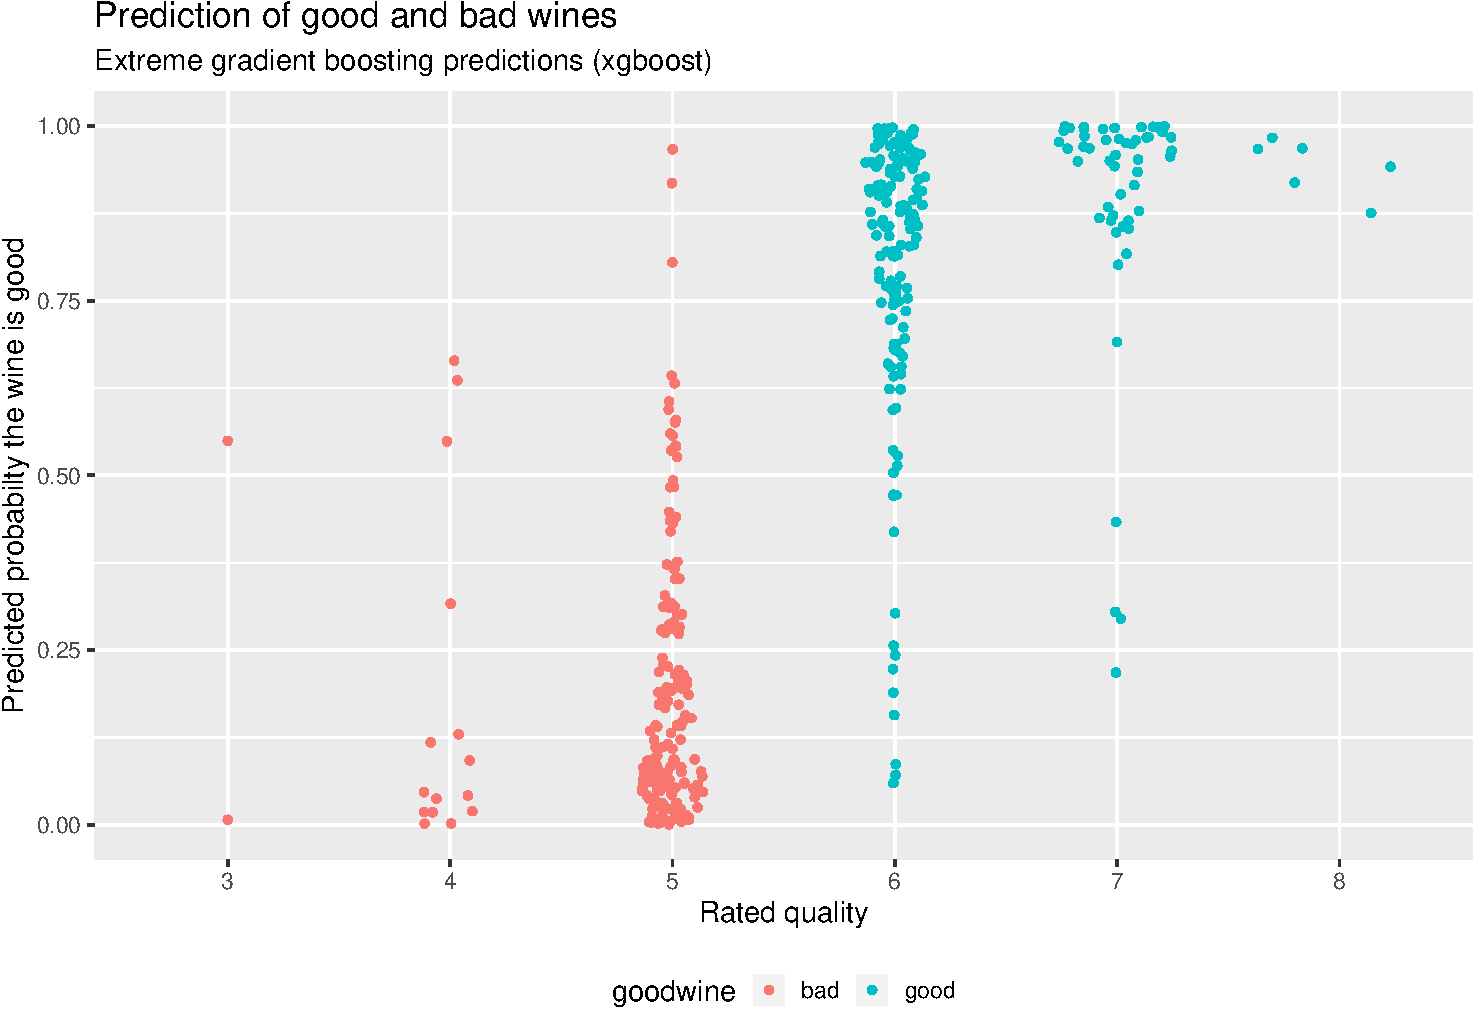
\includegraphics[width=0.9\linewidth]{ML_with_caret_files/figure-beamer/xgb-pred-plot-1}

\end{frame}

\begin{frame}{Assess Variable Importance: glm and xgb}

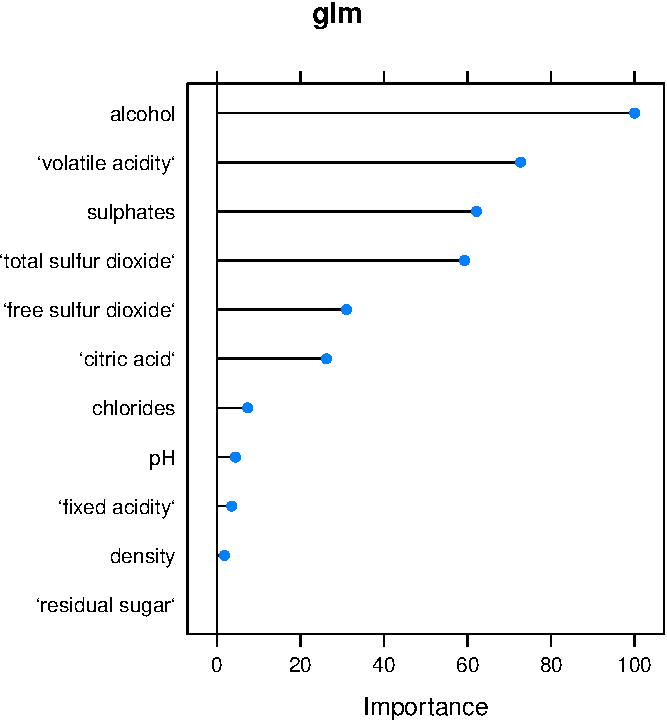
\includegraphics{ML_with_caret_files/figure-beamer/assess-var-glm-1.pdf}

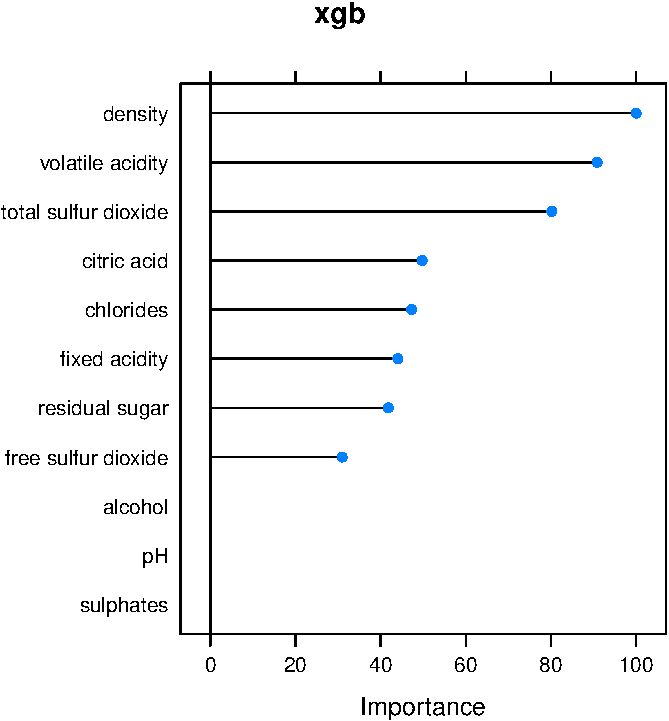
\includegraphics{ML_with_caret_files/figure-beamer/assess-var-xgb-1.pdf}

\end{frame}

\begin{frame}[fragile]{Exercise: Assess model performance and variable
importance}

-- Assess model performance

\texttt{xgb.pred\ =\ predict(xgb.fit,\ testScaled)}

\texttt{confusionMatrix(xgb.pred,\ testClass)}

-- Assess variable importance

\texttt{plot(varImp(xgb.fit,\ scale\ =\ TRUE))}

\end{frame}

\begin{frame}{Addressing the Black Box Problem with Understandable
Models}


\includegraphics[width=0.43\linewidth]{MatrixAlgebraCartoon}

\end{frame}

\begin{frame}[fragile]{An Understandable Model\textbar{}Fast and frugal
decision trees}

\begin{Shaded}
\begin{Highlighting}[]
\KeywordTok{library}\NormalTok{(FFTrees)}
\NormalTok{wine.df =}\StringTok{  }\KeywordTok{read_csv}\NormalTok{(}\StringTok{"winequality-red.csv"}\NormalTok{)}
\NormalTok{wine.df =}\StringTok{ }\NormalTok{wine.df }\OperatorTok\StringTok{ }\KeywordTok{mutate}\NormalTok{(}\DataTypeTok{goodwine =} \KeywordTok{if_else}\NormalTok{(quality}\OperatorTok{>}\DecValTok{5}\NormalTok{, }\OtherTok{TRUE}\NormalTok{, }\OtherTok{FALSE}\NormalTok{)) }\OperatorTok
\StringTok{  }\KeywordTok{select}\NormalTok{(}\OperatorTok{-}\NormalTok{quality)}

\NormalTok{inTrain =}\StringTok{ }\KeywordTok{createDataPartition}\NormalTok{(wine.df}\OperatorTok{$}\NormalTok{goodwine, }\DataTypeTok{p =} \DecValTok{3}\OperatorTok{/}\DecValTok{4}\NormalTok{, }\DataTypeTok{list =} \OtherTok{FALSE}\NormalTok{)}
\NormalTok{train.wine.df =}\StringTok{ }\NormalTok{wine.df[inTrain, ] }
\NormalTok{test.wine.df =}\StringTok{ }\NormalTok{wine.df[}\OperatorTok{-}\NormalTok{inTrain, ]}

\NormalTok{fft.fit =}\StringTok{ }\KeywordTok{FFTrees}\NormalTok{(}\DataTypeTok{formula =}\NormalTok{ goodwine}\OperatorTok{~}\NormalTok{., }\DataTypeTok{data =}\NormalTok{ train.wine.df, }\DataTypeTok{do.comp =} \OtherTok{FALSE}\NormalTok{)}
\end{Highlighting}
\end{Shaded}

\end{frame}

\begin{frame}{Fast and Frugal Decision Tree}

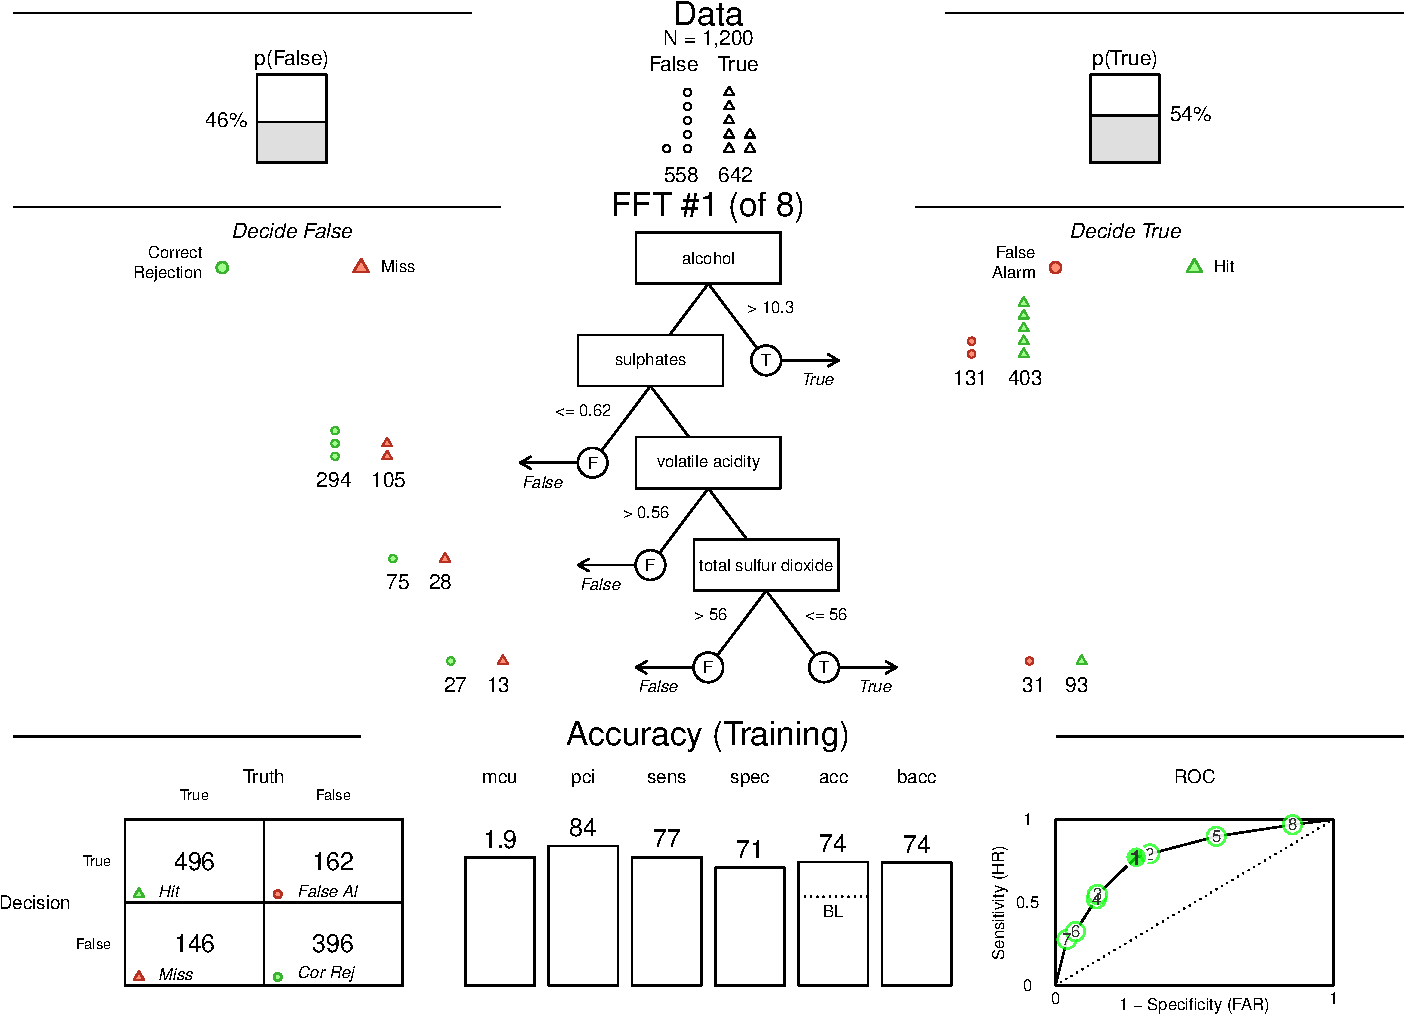
\includegraphics[width=0.9\linewidth]{ML_with_caret_files/figure-beamer/plot_fft-1}

\end{frame}

\begin{frame}{Understandable (fft) and Sophisticated (xgb)}

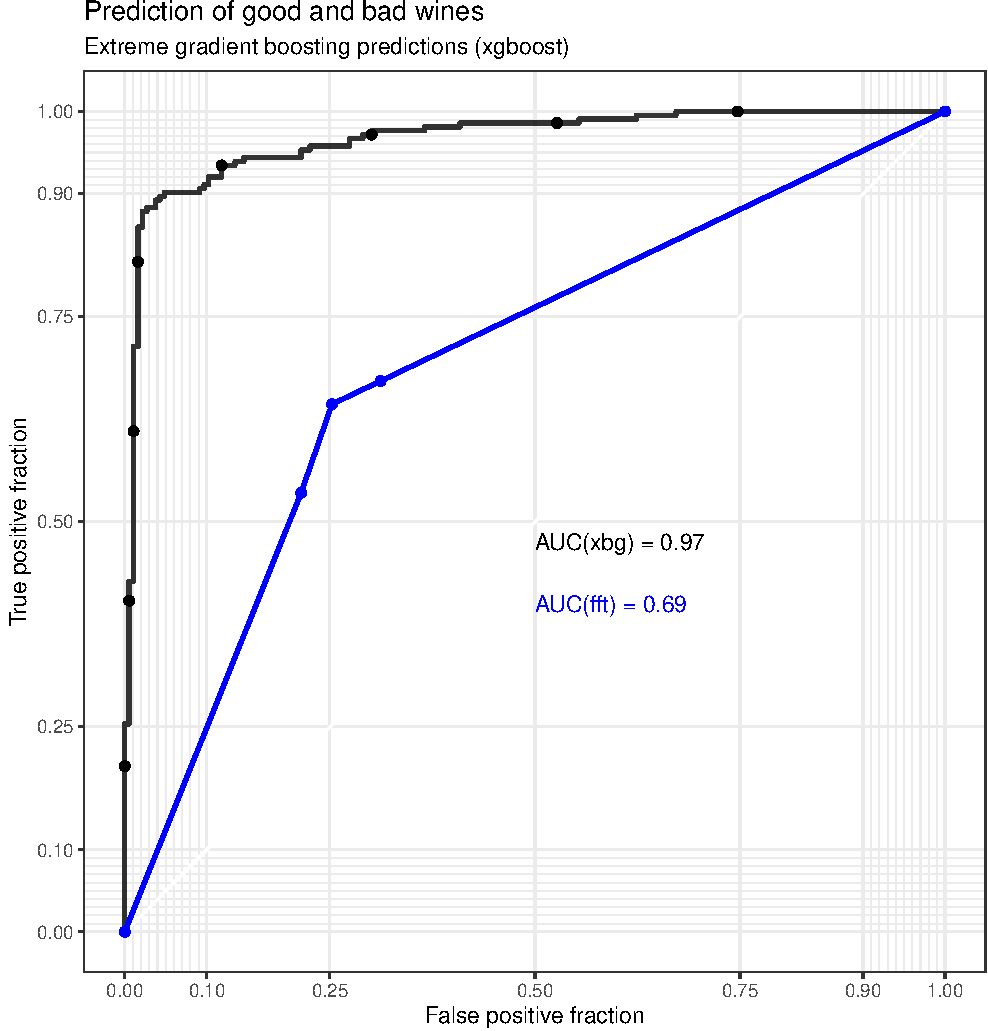
\includegraphics[width=0.95\linewidth]{ML_with_caret_files/figure-beamer/compare_fft_xgb-1}

\end{frame}

\begin{frame}[fragile]{Regression\textbar{}Prediction of continuous
variables}

-- Similar process different performance metrics

\begin{verbatim}
- RMSE--Root mean square error

- MAE--Mean absolute error
\end{verbatim}

-- General issues with model metrics

\begin{verbatim}
- How to penalize the model for large deviations?

- Does the sign of the error matter?

- How to define and ensure fair algorithms?

- Similar to the issue with classificaiton: Are misses and false alarms equally problematic?
\end{verbatim}

 -- Cost sensitive learning and optimal \(\beta\)


\includegraphics[width=0.45\linewidth]{CostSensitveML}

\end{frame}

\begin{frame}{Cross validation: Deploy and monitor}

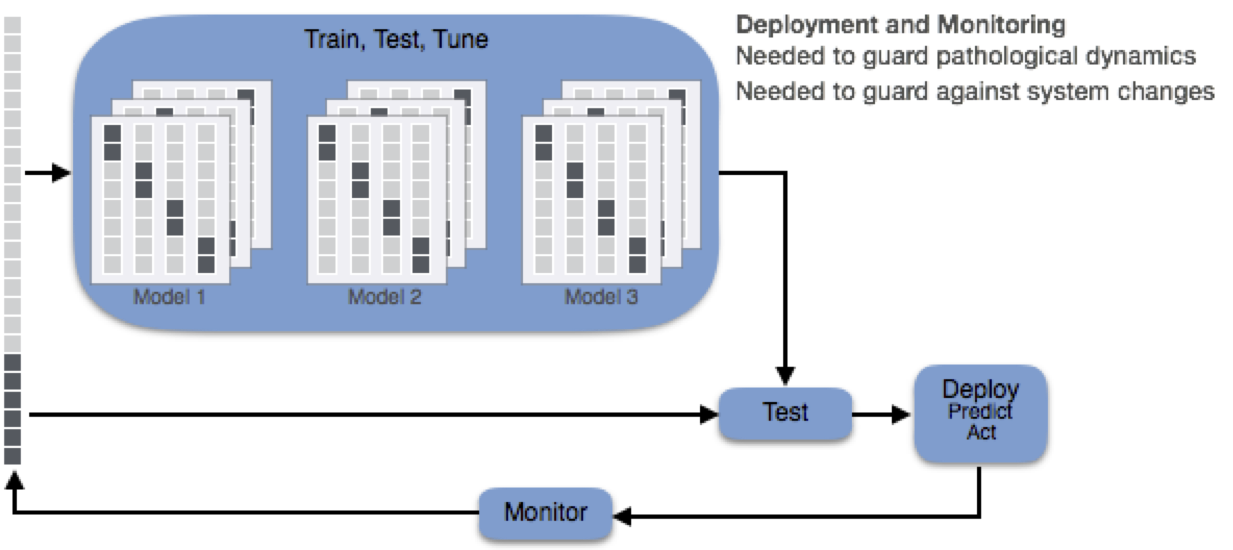
\includegraphics[width=10.28in]{4.DeployMonitor}

\end{frame}

\begin{frame}{Simplified Machine Learning Process}

-- Partition data into training and test sets

-- Pre-process data and select features

-- Tune model hyperparameters with cross validation

-- Estimate variable importance

-- Assess predictions and model performance with test data

-- Compare model performance

\textbf{At each step be sure to model with people in mind}

\end{frame}

\end{document}
